% !TEX root = main.tex
\section{数値実験}

\subsection{課題 1}
\subsubsection{課題内容}
最適化アルゴリズムの評価には,さまざまなテスト関数が利用されている.\textbf{Rastrigin 関数以外}の単一目的関数を調査し,それらの特徴を整理して Python で実装しなさい.

文献\cite{ref4}などを参考にし,最適化アルゴリズムのベンチマーク関数としてよく使用されるテスト関数について調査する.

なお,テスト関数の性質としては以下のような要素がある.

\begin{itemize}
  \item \textbf{単峰性関数(Unimodal functions)}:最適解がただ一つの谷に存在する関数
  \item \textbf{多峰性関数(Multimodal functions)}:最適解が複数の谷に存在する関数
  \item \textbf{変数間の依存関係の有無(Variable dependencies)}:変数が独立しているか,または相互に依存しているか
\end{itemize}

具体的なテスト関数として,次に示す3つの関数を紹介する.これらの関数は最適化問題において広く利用され,それぞれ異なる性質を持っている.

\begin{itemize}
  \item \textbf{Sphere 関数}:この関数は,すべての変数が独立しており,最適解は原点(全ての変数が 0)にある.
  \[
    f_{\mathrm{Sphere}}(x_i) = \sum_{i=1}^{D} x_i^2,\quad (-10 \leq x_i \leq 10) \tag{6}
  \]

  \item \textbf{Rosenbrock 関数(Rosenbrock-Star)}:この関数は,変数間に依存関係がある.
  \[
    f_{\mathrm{Rosenbrock\mbox{-}Star}}(x_i) = \sum_{i=1}^{D-1} \left\{100(x_{i+1} - x_i^2)^2 + (x_i - 1.0)^2 \right\},\quad (-10 \leq x_i \leq 10) \tag{7}
  \]

  \item \textbf{Griewank 関数}:この関数は,複数の変数が相互に影響し合う形式で,非常に多くの局所最小値を持っている.
  \[
    f_{\mathrm{Griewank}}(x_i) = \frac{1}{4000} \sum_{i=1}^{n} x_i^2 - \prod_{i=1}^{n} \cos\left(\frac{x_i}{\sqrt{i}}\right) + 1,\quad (-500 \leq x_i \leq 500) \tag{8}
  \]
\end{itemize}

各関数の特徴を理解し,それぞれ Python で実装する.そして,実装したテスト関数を利用し,PSO で最適化を行いなさい.
\subsubsection{課題結果及び考察}

本課題では,最適化アルゴリズムである粒子群最適化(PSO)を用いて,4種類のベンチマーク関数(Sphere関数,Rosenbrock関数,Griewank関数,Rastrigin関数)に対して最小値探索を行い,それぞれの収束過程を比較・考察した.

図\ref{fig:convergence}に各関数における最良評価値の世代推移を示す.Sphere関数は最も単純な単峰性かつ独立変数型の関数であり,PSOは初期世代から急速に最適解へと収束した.Rastrigin関数およびGriewank関数は多峰性関数であり,多数の局所解を持つにもかかわらず,PSOはそれらを回避して比較的スムーズに収束した.特にGriewank関数では,非常に滑らかな収束曲線が得られており,PSOの探索性能の高さが伺える.

一方,Rosenbrock関数は変数間に強い依存関係を持ち,評価関数の谷が細く曲がっていることから,PSOのような群知能アルゴリズムにとっては収束が困難であることが知られている.本実験においても,初期世代で高い評価値を示し,収束に時間を要していることが確認できた.これはPSOが探索空間の谷に沿って進むのに苦戦している様子を反映していると考えられる.

以上より,PSOは多峰性関数に対しても一定の有効性を示すが,変数間に依存関係がある関数に対しては収束性に課題が残ることが示された.今後は局所探索を補強する手法(例:ハイブリッドアルゴリズム)やパラメータチューニングにより,収束性能の向上が期待される.

\begin{figure}[H]
    \centering
    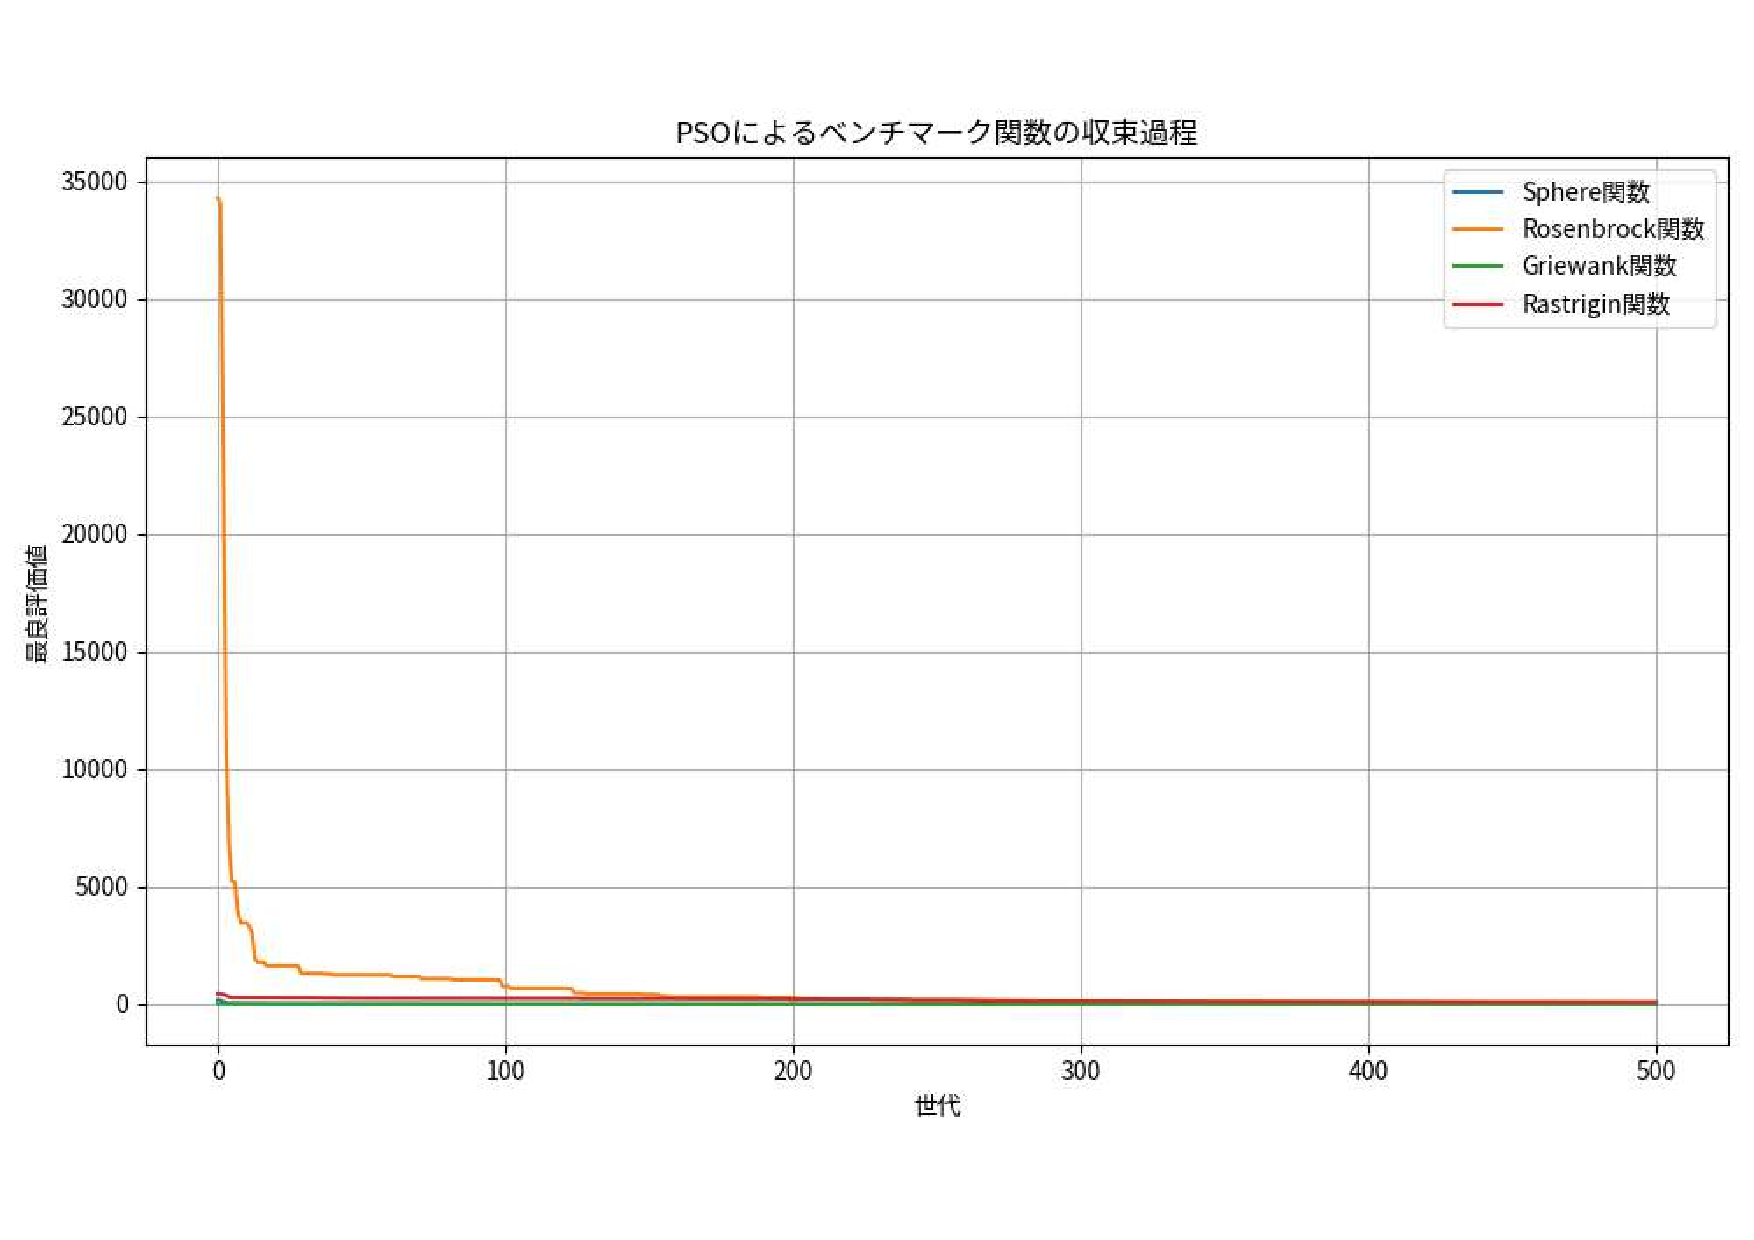
\includegraphics[width=0.8\linewidth]{figure/収束グラフ.pdf}
    \caption{PSOによるベンチマーク関数の収束過程}
    \label{fig:convergence}
\end{figure}

\newpage
\subsubsection{使用したプログラムコード}

\begin{lstlisting}[caption=PSOによるベンチマーク関数の最適化, label=lst:pso_code]
import os
import math
import random
import matplotlib.pyplot as plt
import pandas as pd

# 日本語フォント設定
plt.rcParams['font.family'] = 'Noto Sans CJK JP'

def fitFuncSphere(xVals):
    return sum(x**2 for x in xVals)

def fitFuncRosenbrock(xVals):
    return sum(100 * (xVals[i] - xVals[i-1])**2 + (xVals[i-1] - 1)**2 for i in range(1, len(xVals)))

def fitFuncGriewank(xVals):
    sum_term = sum(x**2 for x in xVals) / 4000
    prod_term = 1
    for i in range(len(xVals)):
        prod_term *= math.cos(xVals[i] / math.sqrt(i + 1))
    return sum_term - prod_term + 1

def fitFuncRastrigin(xVals):
    return 10 * len(xVals) + sum(x**2 - 10 * math.cos(2 * math.pi * x) for x in xVals)

def initPosition(Np, Nd, xMin, xMax):
    return [[xMin + random.random() * (xMax - xMin) for _ in range(Nd)] for _ in range(Np)]

def initVelocity(Np, Nd, vMin, vMax):
    return [[vMin + random.random() * (vMax - vMin) for _ in range(Nd)] for _ in range(Np)]

def updateVelocity(R, V, Np, Nd, j, w, vMin, vMax, pBestPos, gBestPos, c1, c2):
    for p in range(Np):
        for i in range(Nd):
            r1 = random.random()
            r2 = random.random()
            V[p][i] = (w * V[p][i] +
                       c1 * r1 * (pBestPos[p][i] - R[p][i]) +
                       c2 * r2 * (gBestPos[i] - R[p][i]))
            V[p][i] = max(min(V[p][i], vMax), vMin)

def updatePosition(R, V, Np, Nd, xMin, xMax):
    for p in range(Np):
        for i in range(Nd):
            R[p][i] += V[p][i]
            R[p][i] = max(min(R[p][i], xMax), xMin)

def updateFitness(R, M, Np, pBestPos, pBestVal, gBestPos, gBestValue, fitFunc):
    for p in range(Np):
        M[p] = fitFunc(R[p])
        if M[p] < gBestValue:
            gBestValue = M[p]
            gBestPos[:] = R[p][:]
        if M[p] < pBestVal[p]:
            pBestVal[p] = M[p]
            pBestPos[p][:] = R[p][:]
    return gBestValue

def runPSO(fitFunc, name, Np=30, Nd=30, Nt=500,
           xMin=-5.12, xMax=5.12,
           vMin=None, vMax=None,
           wMin=0.4, wMax=0.9, c1=2.05, c2=2.05):

    vMin = vMin if vMin is not None else 0.25 * xMin
    vMax = vMax if vMax is not None else 0.25 * xMax

    R = initPosition(Np, Nd, xMin, xMax)
    V = initVelocity(Np, Nd, vMin, vMax)
    M = [fitFunc(R[p]) for p in range(Np)]
    pBestVal = M[:]
    pBestPos = [r[:] for r in R]
    gBestValue = min(M)
    gBestPos = R[M.index(gBestValue)][:]
    history = [gBestValue]

    for j in range(Nt):
        w = wMax - (wMax - wMin) * j / Nt
        updatePosition(R, V, Np, Nd, xMin, xMax)
        gBestValue = updateFitness(R, M, Np, pBestPos, pBestVal, gBestPos, gBestValue, fitFunc)
        updateVelocity(R, V, Np, Nd, j, w, vMin, vMax, pBestPos, gBestPos, c1, c2)
        history.append(gBestValue)
    
    return name, history

def main():
    output_dir = "./実験1結果"
    os.makedirs(output_dir, exist_ok=True)

    benchmark_funcs = [
        (fitFuncSphere, "Sphere関数"),
        (fitFuncRosenbrock, "Rosenbrock関数"),
        (fitFuncGriewank, "Griewank関数"),
        (fitFuncRastrigin, "Rastrigin関数")
    ]

    all_histories = []
    df_data = {}

    for func, name in benchmark_funcs:
        print(f"{name} のPSO最適化を実行中...")
        name, history = runPSO(func, name)
        all_histories.append((name, history))
        df_data[name] = history

    df = pd.DataFrame(df_data)
    df.index.name = "世代"
    df.to_csv(os.path.join(output_dir, "収束履歴表.csv"))

    plt.figure(figsize=(10, 6))
    for name, history in all_histories:
        plt.plot(history, label=name)
    plt.xlabel("世代")
    plt.ylabel("最良評価値")
    plt.title("PSOによるベンチマーク関数の収束過程")
    plt.legend()
    plt.grid(True)
    plt.tight_layout()
    plt.savefig("figure/収束グラフ.pdf")
    plt.show()

if __name__ == "__main__":
    main()
\end{lstlisting}



\subsection{課題 2}


\subsubsection{課題内容}

\subsubsection{課題結果及び考察}


\subsection{課題 3}


\subsubsection{課題内容}

\subsubsection{課題結果及び考察}


\subsection{課題 4}


\subsubsection{課題内容}

\subsubsection{課題結果及び考察}


\subsection{課題 5}


\subsubsection{課題内容}

\subsubsection{課題結果及び考察}


\subsection{課題 6}


\subsubsection{課題内容}

\subsubsection{課題結果及び考察}


\subsection{課題 7}


\subsubsection{課題内容}

\subsubsection{課題結果及び考察}

